\section{Experimental evaluation} 
\label{experimental_evalutation}
This part assess the solutions put forth in the preceding sections and demonstrate their efficacy in a simulated real-world scenario using data that was generated in a way that reflect reality. The performance of the algorithms explored in this paper have been measured on a machine with the following  specifications: Intel Core i7-6700HQ CPU @ 3.5GHz with 16 GB of RAM.


\subsection{Datasets}
The algorithms that implement the solutions proposed in this research have been tested on several datasets that were artificially constructed to as closely resemble a real-world scenario.
In particular, the synthetic datasets were produced starting with a relational table that was filled with the Scikit-Learn library's \emph{make\_blobs} function, which makes it possible to generate correlated data. The choice of generating correlated data is motivated by the observation that in a real world scenario, in a relational table representing for example people, there exist groups of persons who share characteristics like eye color, height, etc. 

The query set is also built in a realistic manner; precisely, the conditions of each query are constructed by selecting a random number of features (even zero), giving each one a value in the feature's column with a chance of $99$ percent, and using the remaining probability to give a generic random value (even not in the admitted values of that feature). By doing this, the queries are created in a way that causes a great number of them to return some few rows, others to return all the rows, and eventually no rows at all. It's important to note that when a query has no conditions, all of the rows in the relational database are returned. 

The core of the dataset is the utility matrix and to generate this the idea is to create categories of users that are users tend to have the same taste of others. In addition users tends to act following patters. For this reason to fill the utility matrix ratings for the users the idea is to first split the users in three categories:
\begin{enumerate}
    \item $60$ percent of the users rates queries that returns similar rows in the same way. If two queries $q_1$ and $q_2$ returns the majority of the rows in common, the user who rates query $q_1$ with rating $r$ will rate query $q_2$ with a rating that differs by $r$ by a tiny factor $\gamma$, for instance $\gamma = 5$. 
    \item $30$ percent of users grade the queries proportionately with the amount of rows returned by the query. A user may be satisfied when the query returns some rows, but in another sense unsatisfied if the query does not return any row.
    \item the remaining $10$ percent of the users assign random ratings to the queries.
\end{enumerate}

Even though users can evaluate queries on a scale from $1$ to $100$, it is possible that two users will score a query differently in the real world. For example, one user may rate a query positively with a rating of 50, while another may rate the query positively with a rating of $100$. Because of this, the user ratings produced in the previous phase are randomly divided into the following categories: users who rate on a scale of $1$ to $50$, users who rate on a range of $50$ to $100$, $1$ to $100$, etc. Scaling the ratings is a straightforward process that may be carried out using equation \ref{scale_ratings}, where \emph{low} and \emph{high} represent the user's lowest and highest ratings, respectively.  


\begin{equation}
\begin{aligned}
    U_{ij} =  \frac{(\text{high} - \text{low})}{100}  U_{ij} + \text{low}
\end{aligned}
\label{scale_ratings}
\end{equation}




\subsubsection{Synthetic dataset characteristics}
The synthetic dataset is created as previously described using a relational table with $100$ features over a total of $10000$ rows, and in addition, the values of the relational table were filled with integer numbers; this latter choice is wise because, in general, relational tables take values from a specific domain, making representing cities by their names or by a representative integer number equivalent. The dataset is designed to simulate a system with $500$ users who have submitted the DBMS a total of $2000$ queries. Consequently, the utility matrix is composed of $500$ rows and $2000$ columns (queries). Last but not least, a script has been developed to calculate some crucial information from the relational database and the queries, revealing that, out of a total of $2000$ search queries, $721$ produced at least one row, and the average amount of rows returned by these queries is $3311$. 


Even if the numbers appear to be small, they are sufficient to evaluate the effectiveness of the proposed algorithms. They are particularly sufficient to demonstrate how the algorithm's performance improves in various scenarios: this dataset in particular was produced at that scale to enable its division into smaller portions for even more specific experiments. 

\subsubsection{Real dataset}
Relational tables typically contain experimental observations of real data; as a result, the solutions proposed in this work are also evaluated on a dataset in which a real relational table replaces the synthetic one. In this instance, the relational table is taken from the relational database of the 1994 Census Bureau \cite{relational_db}. This dataset is made up of $14$ columns that reflect individual attributes including age, sex, marital status, and income. The original dataset had over $50000$ individuals, however it was scaled down to only include $10000$ individuals in order to measure performance. The other components of the entire dataset are created using the same methodology as the synthetic one, yielding a total of $2000$ queries and $500$ users. In this case the dataset revealed that, out of a total of $2000$ search queries, $908$ produced at least one row, and the average amount of rows returned by these queries is $3649$. 


\subsection{Fast query similarity search with LSH}
\label{fast_sim_search}
This section analyzes the algorithm's initial building block to demonstrate how it performs in comparison to the baseline method for determining query similarity for collaborative filtering. This section specifically aims to demonstrate how the LSH approach, as explained in sections \ref{minhash_section} and \ref{simhash_section}, may significantly improve the naïve solution without LSH of section  \ref{naive_solution}. First, it is shown that using LSH with MinHash reduces the time required to find similar queries for collaborative filtering using the Jaccard similarity as a similarity measure for the queries, and second, it is shown that SimHash with LSH outperforms its corresponding baseline solution, which tries all possible combinations of queries to find the similar ones. Considering the original solutions, the goal of this section is to identify each query's most related queries based on the utility matrix ratings given by the users: without losing generality, the goal is slightly change to locate the most similar query rather than all the $K$ most similar ones. 

\subsubsection{LSH with MinHash}
In this section the LSH MinHash algorithm is compared with its naïve version that computes the Jaccard similarity to find the most similar query. The time efficiency of these two algorithms is compared in two different scenarios: the first involves a changing number of queries with a constant number of users, and the second involves a changing number of users having a constant number of queries. The approach is to divide the dataset used as input into smaller fractions and test the algorithms on those fractions, simulating smaller datasets in the process. In this case of MinHash and Jaccard similarity a dataset with at most $1000$ queries and $500$ users is sufficient to observe the time complexity growth. The plot of Figure \ref{fig:lsh_minhash_queries} reports the execution time of the two methods in a scenario with a constant amount of $500$ users and a variable number of queries. The other scenario is plotted in Figure \ref{fig:lsh_minhash_users} where the number of queries is kept constant at $1000$ queries and the number of users is variable. In both instances, MinHash is set up to generate a signature matrix with $200$ rows, corresponding to a total of $200$ random perturbations; additionally, the LSH bands are configured to have $6$ rows per band, which divides the signature matrix into $33$ bands. 

The two plots in Figures \ref{fig:lsh_minhash_queries} and Figure \ref{fig:lsh_minhash_users} clearly show the time improvements brought by the use of LSH as opposed to computing the similarity between every pair of queries. It is interesting to see that the two approaches perform similarly in the early stages with small datasets, but that one algorithm clearly outperforms the other in scenarios with larger datasets. 


\begin{figure}[h]        
    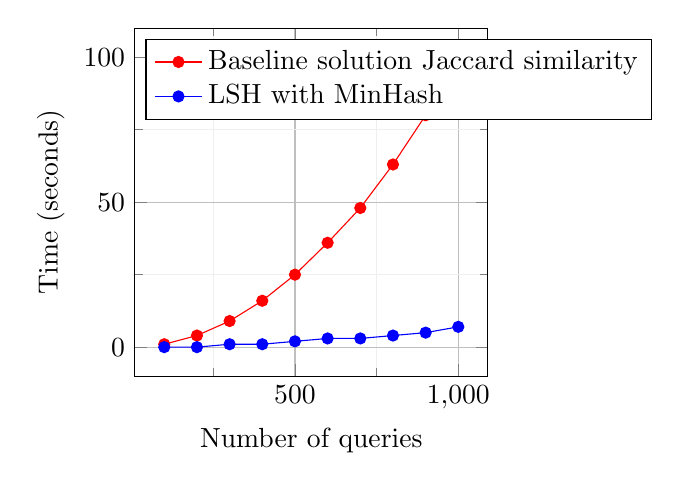
\begin{tikzpicture}
    \begin{axis}[
        xlabel=Number of queries,
        ylabel=Time (seconds),
        height=6cm,
        width = 0.5*\textwidth,
        grid = both,
        minor tick num = 1,
        major grid style = {lightgray},
        minor grid style = {lightgray!25},
        legend cell align = {left},
        legend pos = north west
    ]
    
    % Add values and attributes for the first plot
    \addplot[color=red,mark=*] coordinates {
    	(100, 1)
    	(200, 4)
    	(300, 9)
    	(400, 16)
    	(500, 25)
    	(600, 36)
    	(700, 48)
    	(800, 63)
    	(900, 80)
    	(1000, 100)
    };
    
    % Add values and attributes for the second plot
    \addplot[color=blue,mark=*] coordinates {
    	(100, 0)
    	(200, 0)
    	(300, 1)
    	(400, 1)
    	(500, 2)
    	(600, 3)
    	(700, 3)
    	(800, 4)
    	(900, 5)
    	(1000, 7)
    };
    
    \legend{Baseline solution Jaccard similarity,LSH with MinHash}
    \end{axis}
    \end{tikzpicture}
    
    \caption{\normalfont Time performance of the Naive algorithm compared with LSH using MinHash – Variable number of queries}
    \label{fig:lsh_minhash_queries}
\end{figure}

\begin{figure}[h]
    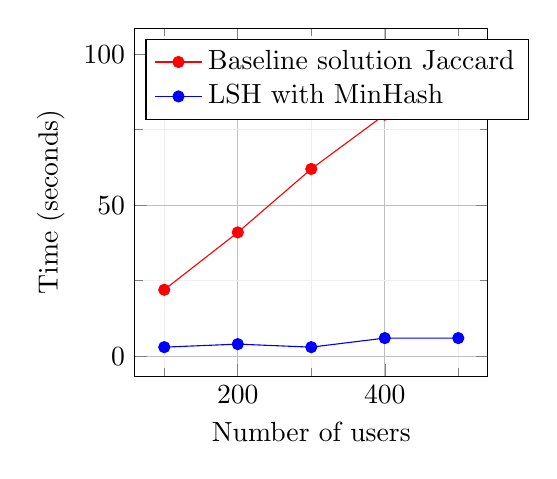
\begin{tikzpicture}
    \begin{axis}[
        xlabel=Number of users,
        ylabel=Time (seconds),
        height=6cm,
        width = 0.5*\textwidth,
        grid = both,
        minor tick num = 1,
        major grid style = {lightgray},
        minor grid style = {lightgray!25},
        legend cell align = {left},
        legend pos = north west
    ]
    
    % Add values and attributes for the first plot
    \addplot[color=red,mark=*] coordinates {
    	(100, 22)
    	(200, 41)
    	(300, 62)
    	(400, 80)
    	(500, 99)
    };
    
    % Add values and attributes for the second plot
    \addplot[color=blue,mark=*] coordinates {
    	(100, 3)
    	(200, 4)
    	(300, 3)
    	(400, 6)
    	(500, 6)
    };
    
    \legend{Baseline solution Jaccard,LSH with MinHash}
    \end{axis}
    \end{tikzpicture}
    \caption{\normalfont Time performance of the Naive algorithm compared with LSH using MinHash – Variable number of users}
    \label{fig:lsh_minhash_users}
\end{figure}



\subsubsection{LSH with SimHash}
The SimHash technique is compared in this section with its naïve counterpart, which computes the cosine similarity between all of the queries in the utility matrix. In this instance, it is possible to observe that leveraging LSH to identify similar queries enhances time performance of the algorithms. 

Given that the naïve approach using the Cosine similarity performs better than the technique using the Jaccard similarity, this time the algorithm is evaluated on a dataset with $2000$ queries rather than $1000$. Furthermore the number of hyperplanes for SimHash has been set at $200$ hyperplanes created at random, corresponding to $200$ rows of the signature matrix; the latter is divided into $13$ bands by LSH increasing the number of rows for each band to $15$. The decision to use a high number of rows per band is due to the fact that SimHash creates a signature matrix of zeros and ones, making it simpler for two queries in the same band to hash in the same bucket. Contrarily, MinHash's signature matrix is made up of integers between $1$ and the entire number of users in the system (rows of the utility matrix), making it less likely that two columns in the same band would hash into the same bucket. 


\begin{figure}[h]        
        
    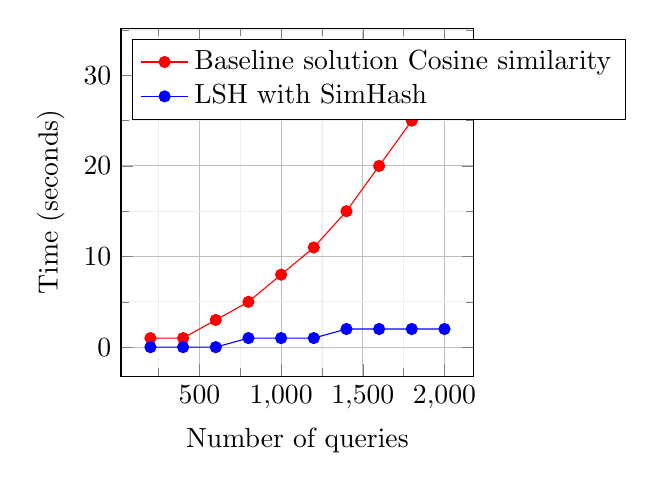
\begin{tikzpicture}
    \begin{axis}[
        xlabel=Number of queries,
        ylabel=Time (seconds),
        height=6cm,
        width = 0.5*\textwidth,
        grid = both,
        minor tick num = 1,
        major grid style = {lightgray},
        minor grid style = {lightgray!25},
        legend cell align = {left},
        legend pos = north west
    ]
    
    % Add values and attributes for the first plot
    \addplot[color=red,mark=*] coordinates {
    	(200, 1)
    	(400, 1)
    	(600, 3)
    	(800, 5)
    	(1000, 8)
    	(1200, 11)
    	(1400, 15)
    	(1600, 20)
    	(1800, 25)
    	(2000, 32)
    };
    
    % Add values and attributes for the second plot
    \addplot[color=blue,mark=*] coordinates {
    	(200, 0)
    	(400, 0)
    	(600, 0)
    	(800, 1)
    	(1000, 1)
    	(1200, 1)
    	(1400, 2)
    	(1600, 2)
    	(1800, 2)
    	(2000, 2)
    };
    
    \legend{Baseline solution Cosine similarity,LSH with SimHash}
    \end{axis}
    \end{tikzpicture}
    
    
    \caption{\normalfont Time performance of the Naive algorithm compared with LSH using SimHash – Variable number of queries}
    \label{fig:lsh_simhash_queries}
\end{figure}


\begin{figure}[h]        
        
    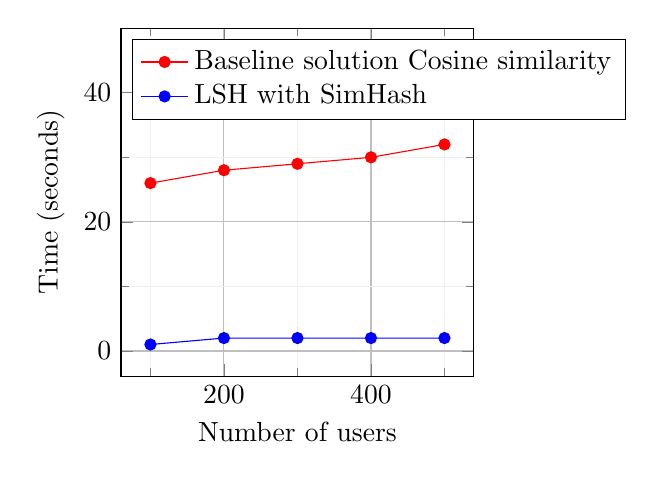
\begin{tikzpicture}
    \begin{axis}[
        xlabel=Number of users,
        ylabel=Time (seconds),
        ymax = 50,
        height=6cm,
        width = 0.5*\textwidth,
        grid = both,
        minor tick num = 1,
        major grid style = {lightgray},
        minor grid style = {lightgray!25},
        legend cell align = {left},
        legend pos = north west
    ]
    
    % Add values and attributes for the first plot
    \addplot[color=red,mark=*] coordinates {
    	(100, 26)
    	(200, 28)
    	(300, 29)
    	(400, 30)
    	(500, 32)
    };
    
    % Add values and attributes for the second plot
    \addplot[color=blue,mark=*] coordinates {
    	(100, 1)
    	(200, 2)
    	(300, 2)
    	(400, 2)
    	(500, 2)
    };
    
    \legend{Baseline solution Cosine similarity,LSH with SimHash}
    \end{axis}
    \end{tikzpicture}
    
    
    \caption{\normalfont Time performance of the Naive algorithm compared with LSH using SimHash – Variable number of users}
    \label{fig:lsh_simhash_queries}
\end{figure}



\subsubsection{LSH parameters tweaks} 
The parameters specifying the size of each LSH band and the number of rows of the signature matrix have a significant impact on LSH performance. Let's study these two characteristics independently in order to better understand their impact. 

\paragraph{Signature matrix rows} The algorithm's time performance will increase as the number of signature matrix's rows decrease, while the probability of finding the wrong most similar query, namely the \emph{error rate}, will decrease as the signature matrix gets smaller. Finding a good balance between the error rate and time performance is crucial, and in border cases it's possible that:
\begin{enumerate}
    \item the error rate is low, meaning the algorithm can accurately predict the queries' most similar queries. The issue with this border case is that LSH will likely discover a set of candidate similar pairs corresponding to all the combinations of queries, which means that the algorithm reverts to the naive approach of trying to find the query that is the most similar by comparing the similarities between all the possible pairs of queries. 
    \item time performance is the best, meaning the algorithm can find the most similar queries quickly. In this case the issue is related to the accuracy of the result, because with a tiny signature matrix, LSH will probably identify too few candidate similar pairs, which increases the likelihood that LSH will miss pairs of queries that may have been similar, i.e. the error rate is large.
\end{enumerate}

The result is clearly depicted in Figures \ref{fig:signature_matrix_rows_error_rate} and Figure \ref{fig:signature_matrix_rows_time} where the test was run using LSH with SimHash configured to divide the signature matrix in bands made of a constant number of $12$ rows. The time the algorithm took to discover the candidate similar queries as well as the error rate were recorded; the error rate is calculated as the complement of the accuracy, i.e. the fraction of successfully predicted most similar queries over all the other queries. 


\begin{figure}[h]        
    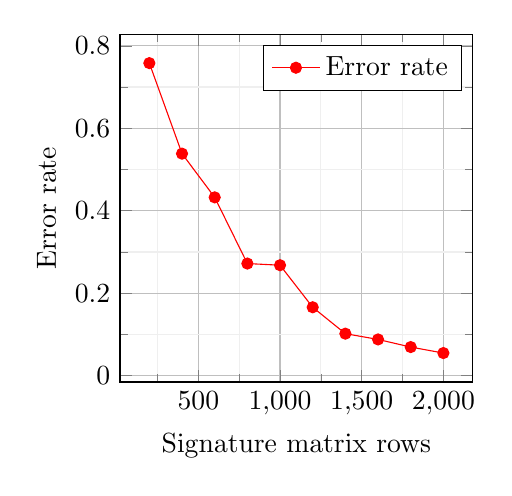
\begin{tikzpicture}
    \begin{axis}[
        xlabel=Signature matrix rows,
        ylabel=Error rate,
        height=6cm,
        width = 0.5*\textwidth,
        grid = both,
        minor tick num = 1,
        major grid style = {lightgray},
        minor grid style = {lightgray!25},
        legend cell align = {left},
        legend pos = north east
    ]
    
    \addplot[color=red,mark=*] coordinates {
    	(200, 0.758)
    	(400, 0.5385)
    	(600, 0.4325)
    	(800, 0.272)
    	(1000, 0.268)
    	(1200, 0.16600000000000004)
    	(1400, 0.10199999999999998)
    	(1600, 0.08799999999999997)
    	(1800, 0.0695)
    	(2000, 0.05500000000000005)
    };
    
    
    \legend{Error rate}
    \end{axis}
    \end{tikzpicture}
    
    \caption{\normalfont As the number of rows in the signature matrix rises, the error rate reduces.}
    \label{fig:signature_matrix_rows_error_rate}
\end{figure}


\begin{figure}[h]        
    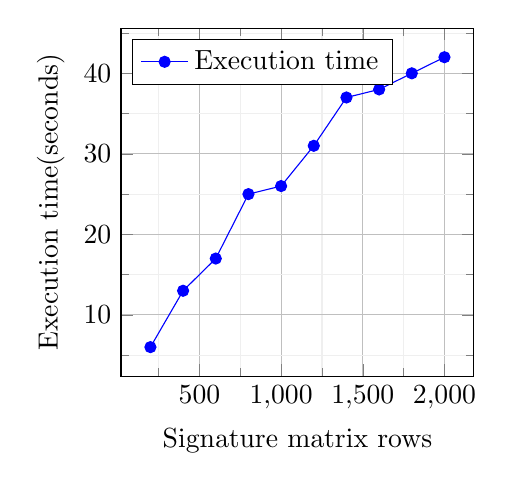
\begin{tikzpicture}
    \begin{axis}[
        xlabel=Signature matrix rows,
        ylabel=Execution time(seconds),
        height=6cm,
        width = 0.5*\textwidth,
        grid = both,
        minor tick num = 1,
        major grid style = {lightgray},
        minor grid style = {lightgray!25},
        legend cell align = {left},
        legend pos = north west
    ]
    
    \addplot[color=blue,mark=*] coordinates {
    	(200, 6)
    	(400, 13)
    	(600, 17)
    	(800, 25)
    	(1000, 26)
    	(1200, 31)
    	(1400, 37)
    	(1600, 38)
    	(1800, 40)
    	(2000, 42)
    };
    
    \legend{Execution time}
    \end{axis}
    \end{tikzpicture}
    
    \caption{\normalfont The time required to search for the most similar query grows as the signature matrix's row count rises.}
    \label{fig:signature_matrix_rows_time}
\end{figure}


\paragraph{LSH band size} As already anticipated also in Section \ref{lsh_description} choosing a good number of rows per band or similarly a number of bands that divides the signature matrix are crucial. In particular in the same way shown for the number of rows of the signature matrix it's possible to observe that testing LSH with SimHash configured to have a constant amount of $200$ signature rows(number of hyperplanes for SimHash) and a variable number of rows per band, when the number of rows for each band increase:
\begin{enumerate}
    \item the error rate tend to increase as shown in Figure \ref{fig:rows_per_band_error_rate}; this is a consequence of the fact that the number of candidate pairs found by LSH decrease.
    \item the algorithm will take less time to find the most similar query as show in Figure \ref{fig:rows_per_band_time}. This is also caused by the fact that LSH only finds a small number of candidate similar pairs of queries, and thus the time required to compare all the possible candidate pairs is less.
\end{enumerate}



\begin{figure}[h]        
    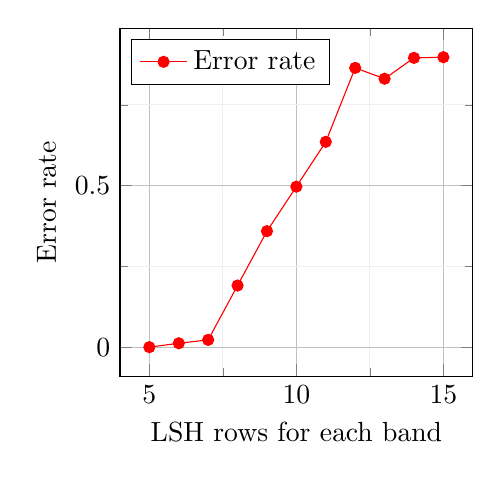
\begin{tikzpicture}
    \begin{axis}[
        xlabel=LSH rows for each band,
        ylabel=Error rate,
        height=6cm,
        width = 0.5*\textwidth,
        grid = both,
        minor tick num = 1,
        major grid style = {lightgray},
        minor grid style = {lightgray!25},
        legend cell align = {left},
        legend pos = north west
    ]
    
    \addplot[color=red,mark=*] coordinates {
        (5, 0.001)
        (6, 0.013)
        (7, 0.023499)
        (8, 0.1915)
        (9, 0.3595)
        (10, 0.497)
        (11, 0.6355)
        (12, 0.864)
        (13, 0.8305)
        (14, 0.895)
        (15, 0.897)
    };
    
    
    \legend{Error rate}
    \end{axis}
    \end{tikzpicture}
    
    \caption{\normalfont As the size of each band rises, the error rate increases.}
    \label{fig:rows_per_band_error_rate}
\end{figure}


\begin{figure}[h]        
    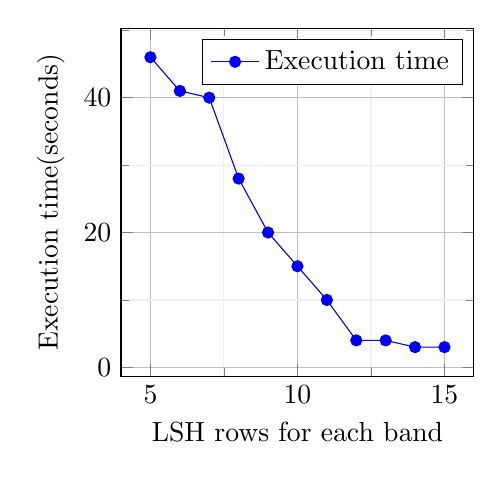
\begin{tikzpicture}
    \begin{axis}[
        xlabel=LSH rows for each band,
        ylabel=Execution time(seconds),
        height=6cm,
        width = 0.5*\textwidth,
        grid = both,
        minor tick num = 1,
        major grid style = {lightgray},
        minor grid style = {lightgray!25},
        legend cell align = {left},
        legend pos = north east
    ]
    
    \addplot[color=blue,mark=*] coordinates {
        (5, 46)
        (6, 41)
        (7, 40)
        (8, 28)
        (9, 20)
        (10, 15)
        (11, 10)
        (12, 4)
        (13, 4)
        (14, 3)
        (15, 3)
    };
    
    \legend{Execution time}
    \end{axis}
    \end{tikzpicture}
    
    \caption{\normalfont The time required to search for the most similar query decreases as the size of each band increases.}
    \label{fig:rows_per_band_time}
\end{figure}


As seen in this section, it is crucial to properly adjust the hyperparameters before executing the algorithm. This should be done while taking into account all possible scenarios. The measurements in this section are calculated by iterating over the various value combinations, measuring the time performance of the process step-by-step, and determining the error as the opposite of accuracy. 

\subsection{Accuracy of the recommendation system}
\label{accuracy_of_rec_sys}
The preceding section analyzed the runtime performance of the algorithm using only collaborative filtering with LSH while tweaking the LSH parameters. However, time performance is not the only aspect that defines a recommendation system's quality. In this section, the accuracy of the algorithms described in this paper is measured using two fundamental metrics: \emph{mean absolute error}(MAE) and \emph{root mean square error}(RMSE). The idea is to compare the accuracy on the following versions of the algorithm:
\begin{enumerate}
    \item Collaborative filtering recommendation system with LSH using MinHash discussed in Section \ref{minhash_section}. 
    \item Collaborative filtering recommendation system with LSH using SimHash discussed in Section \ref{simhash_section}. 
    \item Hybrid recommendation system that combines collaborative filtering(using LSH) with a content based approach as discussed in Section \ref{hybrid_rec_sys_solution}.
    \item Random recommendation system that randomly fills the ratings in the utility matrix.
\end{enumerate}

\subsubsection{MAE and RMSE} The mean absolute error and the root mean squared error have been selected as the two metrics to evaluate the model's accuracy. The distinction between the two is that whereas root mean square error measures the average squared difference between the expected and actual ratings, mean absolute error measures the average difference between the predicted and actual ratings. A high value of RMSE or MAE indicates poor performance in terms of the quality of the recommendation system: both should be lowered to have the maximum accuracy. 

\begin{minipage}{0.49\linewidth}
    \centering
    \begin{equation}
    \label{rmse}
    \begin{aligned}
        MAE = \frac{\sum_i^n \lvert y_i  x_i \lvert }{n}
    \end{aligned}
    \end{equation}
\end{minipage}
\begin{minipage}{0.49\linewidth}
    \centering
    \begin{equation}
    \label{rmse}
    \begin{aligned}
        RMSE = \sqrt{\frac{\sum_i^n (y_i  x_i)^2 }{n}}
    \end{aligned}
    \end{equation}
    
\end{minipage}

\subsubsection{K-fold cross validation}
The idea for measuring the quality of the recommendations, is to apply the K-fold cross validation approach, which takes a portion of non-zero ratings from the utility matrix to be used as a test set, and then runs the aforementioned algorithms on the utility matrix with the ratings in the test set removed. This total procedure is executed $K$ times, where $K=10$ has been selected as a suitable value for the number of folds. The average of the two metrics' accuracy throughout the several folds provides the final indication of MAE and RMSE accuracy. Similar results were obtained using the K-folding approach on both the real dataset and the synthetic dataset, indicating the increase in accuracy that follows from using the content-based strategy of Section \ref{hybrid_rec_sys_solution} to create a hybrid recommendation system. The histograms of Figures \ref{fig:rmse_histo} and \ref{fig:mae_histo} in particular show the average result of the accuracy metrics mentioned above applied on each fold of both the real and synthetic datasets. 

The figures make it clear that the random recommendation system's RMSE and MAE are high in both the datasets, suggesting poor prediction accuracy. The collaborative filtering method is definitely better than the random method, and as the plots demonstrate, the accuracy of the recommendation system increases further when it is combined with a content-based method to form a hybrid recommendation system. The latter is driven by the fact that user ratings are not the only criteria for identifying queries that may be of interest to a user: other aspects of the queries such as the rows they return(their content), are also very important in identifying queries that may be of use to a particular user. 


\begin{figure}[h]        
    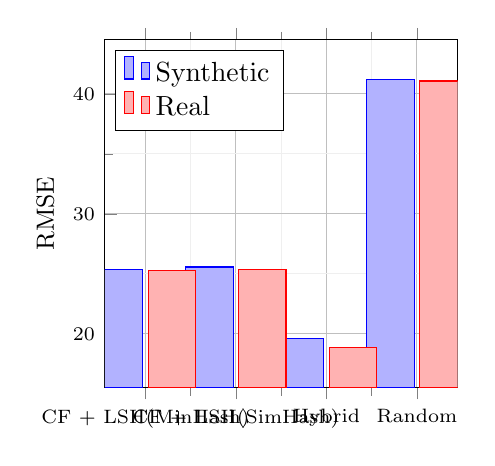
\begin{tikzpicture}
        \begin{axis}[
            enlargelimits=0.15,
            x tick label style={
            /pgf/number format/1000 sep=},
            ylabel={\small{RMSE}},
            width = 0.5*\textwidth, 
            height = 6cm,
            legend pos=north west,
            symbolic x coords={CF + LSH(MinHash), CF + LSH(SimHash), Hybrid, Random},
            xtick=data,
            tick label style={font=\scriptsize},
            ybar,
            bar width = .6cm,
            grid = both,
            minor tick num = 1,
            major grid style = {lightgray},
            minor grid style = {lightgray!25},
            legend cell align = {left},
            legend pos = north west
        ]
        
        \addplot coordinates {(CF + LSH(MinHash),25.390739) (CF + LSH(SimHash),25.575141) (Hybrid,19.596540) (Random,41.166241)};
        \addplot coordinates {(CF + LSH(MinHash),25.248578) (CF + LSH(SimHash),25.365404) (Hybrid,18.864845) (Random,41.073583)};
        
        \legend{Synthetic,Real}
        \end{axis}
    \end{tikzpicture}
    
    \caption{\normalfont Average RMSE of the different algorithms on the two datasets.}
    \label{fig:rmse_histo}
\end{figure}


\begin{figure}[h]        
    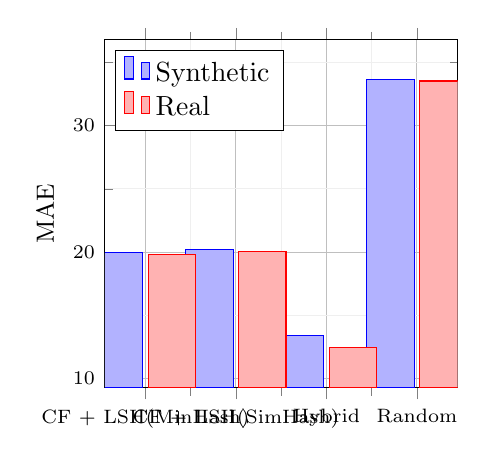
\begin{tikzpicture}
        \begin{axis}[
            enlargelimits=0.15,
            x tick label style={
            /pgf/number format/1000 sep=},
            ylabel={\small{MAE}},
            width = 0.5*\textwidth, 
            height = 6cm,
            legend pos=north west,
            symbolic x coords={CF + LSH(MinHash), CF + LSH(SimHash), Hybrid, Random},
            xtick=data,
            tick label style={font=\scriptsize},
            ybar,
            bar width = .6cm,
            grid = both,
            minor tick num = 1,
            major grid style = {lightgray},
            minor grid style = {lightgray!25},
            legend cell align = {left},
            legend pos = north west
        ]
        
        \addplot coordinates {(CF + LSH(MinHash),19.932730) (CF + LSH(SimHash),20.168860) (Hybrid,13.415692) (Random,33.618878)};
        \addplot coordinates {(CF + LSH(MinHash),19.796775) (CF + LSH(SimHash),20.022409) (Hybrid,12.450330) (Random,33.535856)};
        
        \legend{Synthetic,Real}
        \end{axis}
    \end{tikzpicture}
    
    \caption{\normalfont Average MAE of the different algorithms on the two datasets.}
    \label{fig:mae_histo}
\end{figure}



It's interesting to note that, for all of the algorithms mentioned above, with the exception of the hybrid algorithm, the accuracy metrics produce results that are identical on both datasets, whereas the hybrid recommendation system appears to produce results that are more accurate on the real dataset. This might be related to the data distribution governing the two datasets.


\subsection{Observations}
A recommendation system's quality is determined by a number of essential aspects, including time performance and accuracy. Thanks to the experiments conducted in this section, it is possible to conclude that as model accuracy rises, time performance decreases, and vice versa:
\begin{itemize}
    \item With the random recommendation method, the recommendations are easily calculated and it takes less than one second to fill the utility matrix. However, this approach has the drawback of providing useless recommendations(random).
    \item When LSH and collaborative filtering are combined together, the recommendation system is more accurate compared to random recommendations, however this comes at the expense of a worsening time performance. In addition, as demonstrated in Section \ref{fast_sim_search}, SimHash should be preferred over MinHash on big datasets since it allows for a faster execution time while maintaining the same accuracy for the recommendations: as shown in Section \ref{accuracy_of_rec_sys}, the accuracy of the two LSH techniques is roughly equivalent. 
    \item The collaborative filtering approach relies solely on information derived from user ratings, without considering the characteristics of the queries. This has motivated the integration of a content-based approach with the already-existing collaborative filtering recommendation system described in Section \ref{simhash_section} in order to increase the accuracy of the recommendations. The plots in Section \ref{accuracy_of_rec_sys} demonstrate the accuracy improvement and prove that the hybrid recommendation system works better than the approach employing simply collaborative filtering. However this comes at a higher cost to pay in terms of execution time, in fact computing the item and user profiles is costly and may require several minutes compared to the few seconds needed for collaborative filtering.
\end{itemize}


